\subsection{CDescribeStat类}
CDescribeStat类是\autoref{fig:DesStat}
对话框的关联类,要实现对话框的消息处理和功能程序。
我们为其添加了如下成员函数:
\begin{lstlisting}
public:
	CListCtrl m_ListData; // 数据列表控制变量
	CString m_dbLink; // 储存数据库文件路径
	CString m_sheetName; // 储存输入的表名
	afx_msg void OnBnClickedButtonFile(); // “导入数据库”消息处理
	afx_msg void OnBnClickedButtonBegin(); // “开始统计”消息处理
	afx_msg void OnBnClickedOk(); 
\end{lstlisting}

借助CFileDialog实例来创建打开文件对话框,获取选定文件路径,
然后检验文件合法性。

\begin{figure}[!htbp]
    \centering
    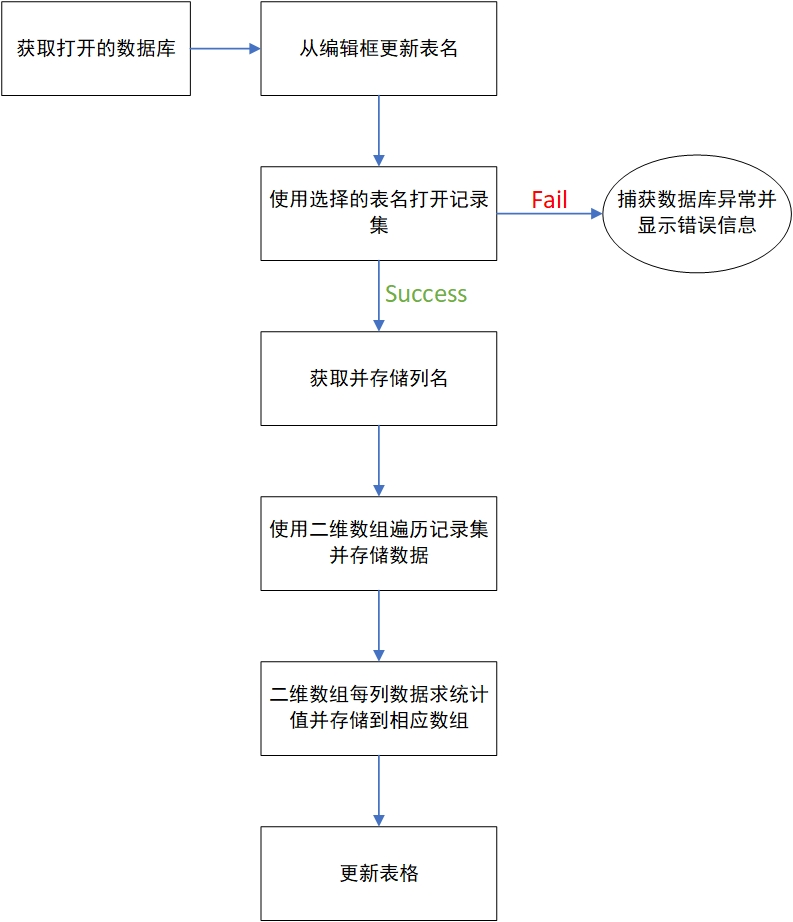
\includegraphics[width = 12cm]{DescribeStat流程图.jpg}
    \caption{程序流程图}
    \label{fig:FlowChart}
\end{figure}

\begin{lstlisting}
    void CDescribeStat::OnBnClickedButtonFile()
    {
        // 创建一个CFileDialog实例
        CFileDialog dlg(TRUE, NULL, NULL, 
            OFN_HIDEREADONLY | OFN_FILEMUSTEXIST, 
            _T("All Files (*.*)|*.*||"));
        // 显示对话框并等待用户响应
        CString dbFilePath;
        if (dlg.DoModal() == IDOK) {
            dbFilePath = dlg.GetPathName(); // 获取选择的文件路径
        }
        m_dbLink = L"DRIVER={Microsoft Access Driver (*.mdb, *.accdb)};DBQ=" + dbFilePath;
        // 检验文件合法性,并打开数据库
        if (db.OpenEx(m_dbLink)) {
            MessageBox(L"成功导入数据库!接下来请填写要统计的表", 
                L"成功", MB_OK);
        }
    }  
\end{lstlisting}
程序功能在OnBnClickedButtonBegin中实现,由于源文件较长,此处
只展示流程图(\autoref{fig:FlowChart}),
其中的二维数组由vector<vector<long double>>实现,详细代码及注释
见附件CDescribeStat.cpp。





